
\chapter{Policy Recommendations and Conclusions}
\begin{flushleft}
Quantitative estimates of Hg emitted into the atmosphere by each country and the corresponding impacts on human health and the environment are crucial for effectively assessing whether legally-binding agreements such as the Minamata Convention (MC) are effective. In such a context, it is evident that quantifying current and future emissions with the best degree of accuracy is an indispensable prerequisite. Consequently, developing and using appropriate methodologies and tools for calculating current emissions and projections within a reasonable uncertainty range is crucial. This chapter aims to provide recommendations on using atmospheric models and monitoring to policymakers in regions with high ASGM incidence to understand ASGM Hg emissions to the atmosphere and its evolution over time. 

\begin{flushleft}
Section \ref{recap} gives a quick summary of the first three chapters. Section \ref{nap_gma18_differences} discusses the discrepancies between GMA 2018 ASGM Hg emission estimates and those in the NAPs. This section aims to underscore the value add that atmospheric monitoring and modeling provide in the presence of such inconsistencies. Moreover, section \ref{motreal_protocol_comparison} uses the Montreal Protocol as an example to discuss the possibilities provided by combining atmospheric monitoring and modeling to inform actions by parties as well as evaluate the effectiveness of the MC. The discussion in this section drives the point that atmospheric monitoring and modeling provides valuable information but may be politically controversial depending on the expectation of parties and the type of penalties imposed on violators of MC's legally binding agreements. Next, section \ref{c4_recommendations} discusses recommendations for governments and policymakers by emphasizing that governments need to prioritize atmospheric monitoring and modeling to understand and combat ASGM Hg emission sources.
% Moreover, I argue that PAS technologies may be the low-hanging fruits that governments roll out as part of the implementation plan since they are affordable and require less skilled technical know-how to set up and maintain. Furthermore, I recommend that countries pursue active regional monitoring by citing Chapter 3 as a sign of what is possible.

\end{flushleft}
\section{Review of First Three Chapters}\label{recap}
This chapter builds upon the results of the first three chapters of this thesis. Chapter one discussed the nature of ASGM activities and their estimated contribution to the global Hg budget. Moreover, challenges regarding knowledge of ASGM Hg emissions were discussed, including the vast uncertainties in ASGM Hg emission estimates. This thesis was partly motivated by the lack of sufficient atmospheric monitoring in most regions where ASGM is prevalent and the absence of modeling studies evaluating Hg emissions from regions with high ASGM emissions. Furthermore, Chapters 2 and 3 showed how data from different Hg atmospheric concentration monitoring technologies could be leveraged and integrated with the GEOS-Chem CTM results to investigate ASGM Hg pollution. Chapter 2 compared the temporal and spatial characteristics of observed and modeled atmospheric Hg concentrations. PAS GEM measurements provided helpful information about the distribution of Hg concentrations across Latin America. Additionally, it was discussed that a network of PAS provides high-quality data while being accessible and affordable to deploy. However, PAS is limited because it does not provide continuous data about atmospheric Hg concentrations. On the other hand, active sampling techniques  such as those conducted by the GMOS Network provided valuable time series data about the atmospheric Hg concentrations. These data enabled broader analysis through the utilization of more metrics to evaluate Hg emissions and better understand temporal variations of Hg concentrations in the atmosphere. By combining active monitoring stations with models, it may be possible to improve understanding of mercury levels in the atmosphere and better define source-receptor relationships. 
\end{flushleft}



\section{Discrepancies Between Global and National ASGM Mercury Estimates}\label{nap_gma18_differences}

According to Evers et al.\cite{evers_evaluating_2016}, country-specific actions under Article 7 of the MC will differ from country to country, and this variability poses a challenge to assessing the MC's effectiveness. Additionally, they argue that understanding changes in the overall use of Hg in the global ASGM sector can be informed by tracking progress in individual countries. They suggest a compilation, visualization, and mapping of the respective data to track this progress across ASGM countries.  The value added by baseline estimates of emissions to policy making is also recognized in the MC's paragraph 3 of Article 7, which stipulates that each party that notifies the secretariat that (ASGM) and processing in its territory is more than insignificant shall develop and implement a national action plan (NAP) per annex C to the MC. In addition, annex C (d) states that the NAP shall include baseline estimates of the quantities of Hg used and the practices employed in ASGM and processing. As of this writing, 18 countries have submitted their respective NAPs. The estimates of how much Hg is used in their territories are shown in Figure\ref{fig:global-hg-emission-estimates_vs_nap_estimates}, which is a bar chart comparing the estimates of annual average Hg emissions predicted in the GMA 2018 inventory in light blue vs. annual average Hg emissions baseline estimates (shown in dark blue) that were reported by the respective countries in their NAPs \cite{united_nations_environment_programme_technical_2019}.

\begin{figure}[H]
  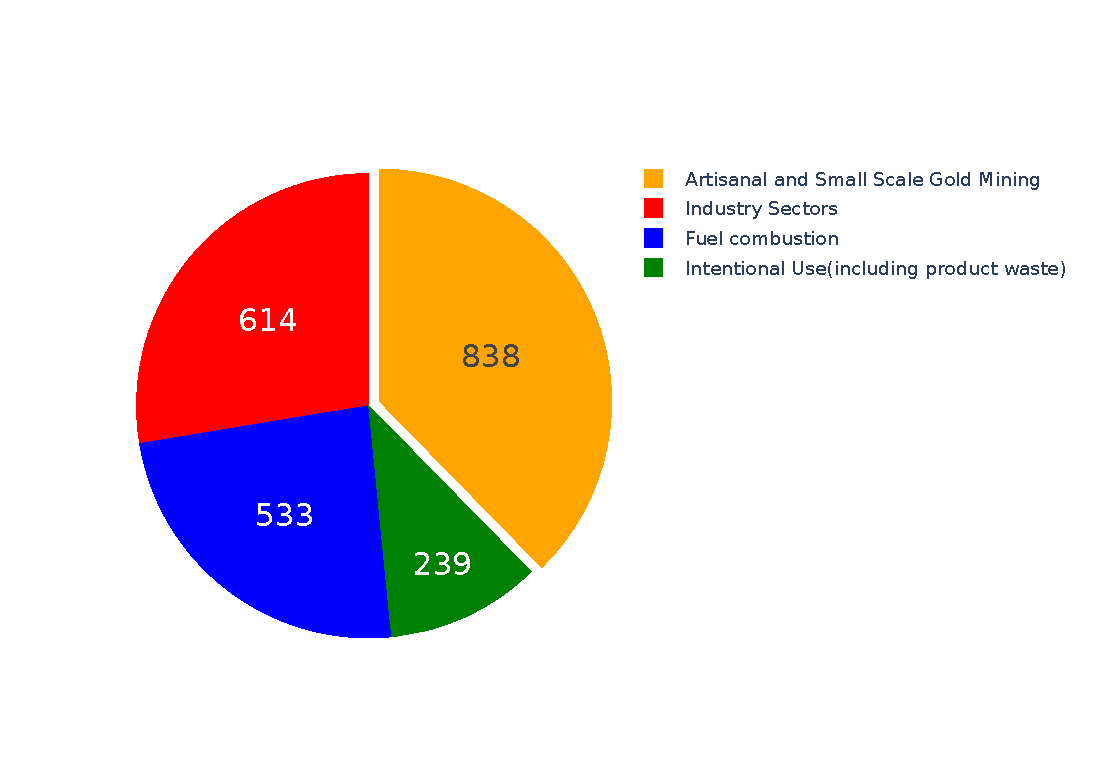
\includegraphics[width=\textwidth]{templates/figures/07-24-22_global-hg-emission-estimates_vs_nap_estimates.pdf}
  \centering
  \caption[Bar chart comparing the  GMA 2018 ASGM Hg emission estimates to NAP baseline ASGM Hg emissions estimates]{Bar chart comparing the estimates of annual average Hg emissions predicted in the GMA 2018 inventory in light blue vs. annual average Hg emissions baseline estimates (shown in dark blue) that were reported by the respective countries in their NAPs \cite{united_nations_environment_programme_technical_2019} }
  \label{fig:global-hg-emission-estimates_vs_nap_estimates}
\end{figure}
\FloatBarrier
\begin{flushleft}
 In Figure \ref{fig:global-hg-emission-estimates_vs_nap_estimates}, it is evident that the difference between the global estimates and the NAP estimates is vast for some countries. While the baseline estimates of Hg use in ASGM as reported in the NAPs and global inventories are critical, data from monitoring networks combined with atmospheric models provide additional tools to evaluate the changes in Hg in the atmosphere. The differences in the estimates do not necessarily indicate emission increases, but they reflect the uncertainties in the global emission estimates. 
\end{flushleft} 

\section{Informing the Use of Atmospheric Modeling for Quantifying ASGM Emissions in the Minamata Convention through Experiences from the Montreal Protocol} \label{motreal_protocol_comparison}

\begin{flushleft}
Monitoring atmospheric concentrations of pollutants of interest and using atmospheric models to understand the data has been critical in evaluating global legally-binding environmental agreements such as the Montreal Protocol. For instance, Rigby et al. 2019 showed how vital the combination of atmospheric monitoring networks and modeling is when they quantified the amount of an observed increase in CFC-11 and identified where the source was located\cite{rigby_increase_2019}. They used high-frequency atmospheric observations from Gosan, South Korea, and Hateruma, Japan, and global monitoring data and atmospheric CTM simulations to investigate regional CFC-11 emissions from eastern Asia.  
\end{flushleft}
\begin{flushleft}
    The above example about the Montreal protocol showcases the multiple benefits of atmospheric monitoring and modeling. For instance, Rigby et al.\cite{rigby_increase_2019}  showed that emissions from eastern mainland China were 7.0 ± 3.0 (±1 standard deviation) gigagrams per year higher in 2014–2017 than in 2008–2012 and that the increase in emissions arose primarily around the northeastern provinces of Shandong and Hebei\cite{rigby_increase_2019}. This kind of precision of emission estimates and the approximate location of their sources would be beneficial for evaluating the effectiveness of MC efforts aimed at reducing Hg emissions. Policymakers would value such information because it would give them precise data about the amounts of emissions and where they should look for the sources. However, it is uncertain if this level of precision could be achieved for an emission source like ASGM, given that it is not a point source.
    
    Another critical aspect of the information provided by the approach discussed in this thesis is the ability to determine areas that have a low likelihood of being sources of increase in emissions. This benefit was also demonstrated  by Rigby et al. (2019)  in that they could conclude that there was no evidence for a significant rise in CFC-11 emissions from any other eastern Asian countries or other regions of the world where there are available data for the detection of regional emissions.
\end{flushleft}

\begin{flushleft}
A look at China's response to scientific information about its increased CFC emissions in the Montreal Protocol example above may provide insight into possible answers by parties when they are notified about emission violations within their territory. China questioned the conclusions of the scientific study noting significant uncertainty. However, they also acknowledged the importance of atmospheric monitoring. They developed a plan to establish a national monitoring network, including substantial penalties for companies that produce insulation foam for ozone-depleting chemicals illegally. Considering that ASGM occurs mainly in poor communities in countries in the global south, the Minamata Convention may need to develop a different strategy for helping countries respond to sudden increases in their ASGM emission sources. For instance, PAS technologies could be deployed at locations of interest once regional active monitoring networks and models have identified spikes in ASGM Hg emissions. Lawmakers should rely on legal measures to curb emissions, such as banning mercury or restricting ASGM communities as a last resort. These types of command-and-control strategies have been shown to dissuade miners from cooperating.
\end{flushleft}


% \section{Current Perspectives on Applications of Atmospheric Monitoring and Modeling to Evaluate the Effectiveness of the Minamata Convention in Combating ASGM Emissions}

%  The necessity of atmospheric Hg monitoring for evaluating the MC is clearly expressed in the report published by the MC secretariat about the guidance on tracking mercury and mercury compounds to support the assessment of the effectiveness of the Minamata Convention\cite{unep_guidance_2021}. Also, the proposed indicators for evaluating the effectiveness of the Minamata Convention on Mercury show the level of trust that parties have in science and the use of monitoring data and atmospheric models.

\section{Recommendations}\label{c4_recommendations}
% \subsection{Governments and Policy Makers}

As part of monitoring ASGM activities and defining policy related to ASGM activities, government officials and policymakers are encouraged to include atmospheric monitoring.  Governments may be able to set up monitoring within their territories by using PAS technologies. Moreover, governments are encouraged to establish regional active monitoring stations in collaboration at the regional level. According to chapter three, a reasonable estimation of emissions can be made based on data from one station. In this way, a few regional active monitoring networks and widespread national PAS networks may prove helpful for evaluating the effectiveness of MC activities.
  
The monitoring of atmospheric Hg can provide information about ASGM activities and help identify them. As a result, these data can be used to establish a baseline of mercury use in ASGM and to evaluate policies related to reducing it. Through cartographic and statistical products, monitoring and modeling outputs can be understandable to non-technical audiences, thus facilitating artisanal mining policy development. 

Modeling the atmosphere using CTMs requires technical skills not usually available in government agencies or policy agencies because it requires technical competencies typically found in scientific communities. Consequently, investing in capacity building among mining administrations lacking technical knowledge and soliciting researchers' know-how from local universities are critical recommendations for government officials and policymakers.  
 
It is necessary to consider that technical competency is not always present in local communities and mining associations. As a result, their involvement in monitoring programs and policy development may be reduced or compromised. Tensions can sometimes be exacerbated by this, which undermines local trust. Therefore, government officials and policymakers should include local communities and artisanal miners when developing ASGM policies and programs. 


\section{Conclusion}
\begin{flushleft}
In this chapter, I compared the GMA 2018 estimates to the estimates that countries have provided in their NAPs to highlight the value that atmospheric monitoring the modeling would add to the policy-making process. Moreover, experiences from the Montreal Protocol were referenced to discuss the point that atmospheric monitoring and modeling provides valuable information but may be politically controversial depending on the expectation of parties. Finally, I recommended that countries pursue regional active monitoring  referencing the third chapter of this thesis as a source of insight into the value that one site provides. 
\end{flushleft}